 % !TEX encoding = UTF-8 Unicode
% !TeX TXS-program:compile = txs:///pdflatex/[--shell-escape] 

\documentclass[12pt, twoside]{book}
%***************************************************************************************************

% Podstawowe ustawienia języka, według którego formatowany będzie dokument
%\usepackage[english,polish]{babel}
\usepackage[english]{babel}

% Pakiet babel dla polskiego języka powoduje konflikt z pakietem amssymb.
% Polecenie '\lll' definiują oba pakiety - porządana jest druga definicja.
\let\lll\undefined

% W przypadku wielojęzykowości ustawia główny język dokumentu
\selectlanguage{english}

% Kodowanie dokumentu
\usepackage[utf8]{inputenc} 
\usepackage[T1]{fontenc} 

% Dowolny rozmiar czcionek, kodowanie znaków
\usepackage{lmodern}

% Polskie wcięcia akapitów
\usepackage{indentfirst}

% Polskie formatowanie typograficzne
\frenchspacing

% Zapewnia liczne usprawnienia wyświetlania i organizacji matematycznych formuł. 
\usepackage{amsmath}

% Wprowadza rozszerzony zestaw symboli m.in. \leadsto
\usepackage{amssymb}

% Dodatkowa, ,,kręcona'' czcionka matematyczna
\usepackage{mathrsfs}

% Dodatkowe wsparcie dla środowiska mathbb, które nie wspiera domyślnie cyfr (\mathbb{})
%\usepackage{bbold}

% Fixes/improves amsmath
\usepackage{mathtools}


% ***************************************************************************************************
% Kolory  
% ***************************************************************************************************

% Umożliwia kolorowanie poszczególnych komórek tabeli
\usepackage[table, svgnames]{xcolor}% http://ctan.org/pkg/

% Umożliwia łatwą zmianę koloru linii w tabeli
\usepackage{tabu}

% Umożliwia rozszerzoną kontrolę nad kolorami.
\usepackage{xcolor}

% Definicje kolorów
\definecolor{lgray}{HTML}{9F9F9F}
\definecolor{dgray}{HTML}{5F5F5F}

% ***************************************************************************************************
% Algorytmy 
% ***************************************************************************************************

% Udostępnia środowisko do konstruowania pseudokodów
\usepackage[ruled,vlined,linesnumbered,longend,algochapter]{algorithm2e}

% Zamiana nazwy środowiska z domyślnej "Algorithm X" na "Pseudokod X"
\newenvironment{algorithm-custom}[1][htb]{
	\renewcommand{\algorithmcfname}{Algorithm}
	\begin{algorithm}[#1]%
	}{
\end{algorithm}
}

% Zmiana rozmiaru komentarzy
\newcommand\algcomment[1]{
	\footnotesize{#1}
}

% Ustawienie zadanego stylu dla komentarzy
\SetCommentSty{algcomment}

% Wyśrodkowana tylda
\usepackage{textcomp}%
\newcommand{\textapprox}{\raisebox{0.5ex}{\texttildelow}}

% Listowanie kodów źródłowych
\usepackage{listings} 
\renewcommand{\lstlistingname}{Source code} % Polska nazwa listingu

% ***************************************************************************************************
% Marginesy 
% ***************************************************************************************************

% Ustawienia rozmiarów stron i ich marginesów
\usepackage[headheight=18pt, top=25mm, bottom=25mm, left=25mm, right=25mm]{geometry}

% Usunięcie górnego marginesu dla środowisk
\makeatletter
\setlength\@fptop{0\p@}	
\makeatother

% ***************************************************************************************************
% Styl 
% ***************************************************************************************************

% Definiuje środowisko 'titlingpage', które zapewnia pełną kontrolę nad układem strony tytułowej.
\usepackage{titling}

% Umożliwia modyfikowanie stylu spisu treści
\usepackage[subfigure]{tocloft}	

\tocloftpagestyle{tableOfContentStyle}

% Definiowanie własnych stylów nagłówków i/lub stopek
\usepackage{fancyhdr}

% Domyślny styl dla pracy 
\fancypagestyle{custom}{
	\fancyhf{}									% wyczyść stopki i nagłówki
	\fancyhead[RO]{								% Prawy, nieparzysty nagłówek
		\hrulefill \hspace{16pt} \large Chapter \thechapter
		\put(-471.5,5.5){%
			\makebox(0,0)[l]{%
				\small Wrocław University of Science and Technology
			}
		}
	}
	\fancyhead[LE]{								% Lewy, parzysty nagłówek
		\large Chapter \thechapter \hspace{16pt} \hrulefill 
		\put(-267,5.5){%
			\makebox(0,0)[l]{%
				\small Faculty of Information and Communication Technology
			}
		}
	}
	\fancyfoot[LE,RO]{							% Stopki
		\thepage
	}
	\renewcommand{\headrulewidth}{0pt}			% Grubość linii w nagłówku
	\renewcommand{\footrulewidth}{0.2pt}		% Grubość linii w stopce
}

% Domyślny styl dla List of Figures
\fancypagestyle{ListofFiguresStyle}{
	\fancyhf{}									% wyczyść stopki i nagłówki
	\fancyhead[RO]{								% Prawy, nieparzysty nagłówek
		\hrulefill \hspace{16pt} \large List of Figures
		\put(-471.5,5.5){%
			\makebox(0,0)[l]{%
				\small Wrocław University of Science and Technology
			}
		}
	}
	\fancyhead[LE]{								% Lewy, parzysty nagłówek
		\large List of Figures \hspace{16pt} \hrulefill 
		\put(-267,5.5){%
			\makebox(0,0)[l]{%
				\small Faculty of Information and Communication Technology
			}
		}
	}
	\fancyfoot[LE,RO]{							% Stopki
		\thepage
	}
	\renewcommand{\headrulewidth}{0pt}			% Grubość linii w nagłówku
	\renewcommand{\footrulewidth}{0.2pt}		% Grubość linii w stopce
}

% Domyślny styl dla List of Tables
\fancypagestyle{ListofTablesStyle}{
	\fancyhf{}									% wyczyść stopki i nagłówki
	\fancyhead[RO]{								% Prawy, nieparzysty nagłówek
		\hrulefill \hspace{16pt} \large List of Tables
		\put(-471.5,5.5){%
			\makebox(0,0)[l]{%
				\small Wrocław University of Science and Technology
			}
		}
	}
	\fancyhead[LE]{								% Lewy, parzysty nagłówek
		\large List of Tables \hspace{16pt} \hrulefill 
		\put(-267,5.5){%
			\makebox(0,0)[l]{%
				\small Faculty of Information and Communication Technology
			}
		}
	}
	\fancyfoot[LE,RO]{							% Stopki
		\thepage
	}
	\renewcommand{\headrulewidth}{0pt}			% Grubość linii w nagłówku
	\renewcommand{\footrulewidth}{0.2pt}		% Grubość linii w stopce
}


% Domyślny styl dla bibliografii
\fancypagestyle{bibliographyStyle}{
	\fancyhf{}									% wyczyść stopki i nagłówki
	\fancyhead[RO]{								% Prawy, nieparzysty nagłówek
		\hrulefill \hspace{16pt} \large Bibliography
		\put(-471.5,5.5){%
			\makebox(0,0)[l]{%
				\small Wrocław University of Science and Technology
			}
		}
	}
	\fancyhead[LE]{								% Lewy, parzysty nagłówek
		\large Bibliography \hspace{16pt} \hrulefill 
		\put(-267,5.5){%
			\makebox(0,0)[l]{%
				\small Faculty of Information and Communication Technology
			}
		}
	}
	\fancyfoot[LE,RO]{							% Stopki
		\thepage
	}
	\renewcommand{\headrulewidth}{0pt}			% Grubość linii w nagłówku
	\renewcommand{\footrulewidth}{0.2pt}		% Grubość linii w stopce
}

% Domyślny styl dla dodatków
\fancypagestyle{appendixStyle}{
	\fancyhf{}									% wyczyść stopki i nagłówki
	\fancyhead[RO]{								% Prawy, nieparzysty nagłówek
		\hrulefill \hspace{16pt} \large Appendix \thechapter
		\put(-472.1, 12.1){%
			\makebox(0,0)[l]{%
				\includegraphics[width=0.05\textwidth]{resources/pwr-logo}
			}
		}
		\put(-443,5.5){%
			\makebox(0,0)[l]{%
				\small Wrocław University of Science and Technology
			}
		}
	}
	\fancyhead[LE]{								% Lewy, parzysty nagłówek
		\large Dodatek \thechapter \hspace{16pt} \hrulefill 
		\put(-22, 12.1){%
			\makebox(0,0)[l]{%
				\includegraphics[width=0.05\textwidth]{wiz-logo}
			}
		}
		\put(-220,5.5){%
			\makebox(0,0)[l]{%
				\small Faculty of Information and Communication Technology
			}
		}
	}
	\fancyfoot[LE,RO]{							% Stopki
		\thepage
	}
	\renewcommand{\headrulewidth}{0pt}			% Grubość linii w nagłówku
	\renewcommand{\footrulewidth}{0.2pt}		% Grubość linii w stopce
}


% Osobny styl dla stron zaczynających rozdział/spis treści itd. (domyślnie formatowane jako "plain")
\fancypagestyle{chapterBeginStyle}{
	\fancyhf{}%
	\fancyfoot[LE,RO]{
		\thepage
	}
	\renewcommand{\headrulewidth}{0pt}
	\renewcommand{\footrulewidth}{0.2pt}
}

% Styl dla pozostałych stron spisu treści
\fancypagestyle{tableOfContentStyle}{
	\fancyhf{}%
	\fancyfoot[LE,RO]{
		\thepage
	}
	\renewcommand{\headrulewidth}{0pt}
	\renewcommand{\footrulewidth}{0.2pt}
}

% Formatowanie tytułów rozdziałów i/lub sekcji
\usepackage{titlesec}


% Formatowanie tytułów rozdziałów
\titleformat{\chapter}[hang]
{\vspace{-10ex}\normalfont\Huge\bfseries}											
{\thechapter.}
{1ex}
{} 
%[\vspace{2ex}]

% Formatowanie tytułów sekcji
\titleformat{\section}[hang]
{\normalfont\Large\bfseries}											
{\thesection.}
{1ex}
{} 

\titleformat{\subsection}[hang]
{\normalfont\large\bfseries}											
{\thesubsection.}
{1ex}
{} 
% formatowanie elementów przed modyfikowanym tytułem


% ***************************************************************************************************
% Linki
% ***************************************************************************************************

% Umożliwia wstawianie hiperłączy do dokumentu
\usepackage{hyperref}							% Aktywuje linki

\hypersetup{
	colorlinks	=	true,					% Koloruje tekst zamiast tworzyć ramki.
	linkcolor	=	blue,					% Kolory: referencji,
    citecolor	=	blue,					% cytowań,
	urlcolor	=	blue					% hiperlinków.
}

% Do stworzenia hiperłączy zostanie użyta ta sama (same) czcionka co dla reszty dokumentu
\urlstyle{same}


% ***************************************************************************************************
% Linki
% ***************************************************************************************************

% Umożliwia zdefiniowanie własnego stylu wyliczeniowego
\usepackage{enumitem}

% Nowa lista numerowana z trzema poziomami
\newlist{myitemize}{itemize}{3}

% Definicja wyglądu znacznika pierwszego poziomu
\setlist[myitemize,1]{
	label		=	\textbullet,
	leftmargin	=	4mm}

% Definicja wyglądu znacznika drugiego poziomu
\setlist[myitemize,2]{
	label		=	$\diamond$,
	leftmargin	=	8mm}

% Definicja wyglądu znacznika trzeciego poziomu
\setlist[myitemize,3]{
	label		=	$\diamond$,
	leftmargin	=	12mm
}

% ***************************************************************************************************
% Inne pakiety
% ***************************************************************************************************

% Dołączanie rysunków
\usepackage{graphicx}

% Figury i przypisy
\usepackage{caption}
%\usepackage{subcaption}

% Umożliwia tworzenie przypisów wewnątrz środowisk
\usepackage{footnote}

% Umożliwia tworzenie struktur katalogów
\usepackage{dirtree}

% Rozciąganie komórek tabeli na wiele wierszy
\usepackage{multirow}

% Precyzyjne obliczenia szerokości/wysokości dowolnego fragmentu wygenerowanego przez LaTeX
\usepackage{calc}

% ***************************************************************************************************
% Matematyczne skróty
% ***************************************************************************************************

% Skrócony symbol liczb rzeczywistych
\newcommand{\RR}{\mathbb{R}}

% Skrócony symbol liczb naturalnych
\newcommand{\NN}{\mathbb{N}}

% Skrócony symbol liczb wymiernych
\newcommand{\QQ}{\mathbb{Q}}

% Skrócony symbol liczb całkowitych
\newcommand{\ZZ}{\mathbb{Z}}

% Skrócony symbol logicznej implikacji
\newcommand{\IMP}{\rightarrow}

% Skrócony symbol  logicznej równoważności
\newcommand{\IFF}{\leftrightarrow}

% ***************************************************************************************************
% Środowiska
% ***************************************************************************************************

% Środowisko do twierdzeń
\newtheorem{theorem}{Twierdzenie}[chapter]

% Środowisko do lematów
\newtheorem{lemma}{Lemat}[chapter]

% Środowisko do przykładów
\newtheorem{example}{Przykład}[chapter]

% Środowisko do wniosków
\newtheorem{corollary}{Wniosek}[chapter]

% Środowisko do definicji
\newtheorem{definition}{Definicja}[chapter]

% Środowisko do dowodów
\newenvironment{proof}{
	\par\noindent \textbf{Dowód.}
}{
\begin{flushright}
	\vspace*{-6mm}\mbox{$\blacklozenge$}
\end{flushright}
}

% Środowisko do uwag
\newenvironment{remark}{
	\bigskip \par\noindent \small \textbf{Uwaga.}
}{
\begin{small}
	\vspace*{4mm}
\end{small}
}

% dodatkowe pomagające, oczywiście nie wszystskie są wymagane
\usepackage{psfrag}
\usepackage{amsfonts}
\usepackage{supertabular}
\usepackage{array}
\usepackage{tabularx}
\usepackage{hhline}
\usepackage{minted}
\usepackage{url}
\usepackage{microtype}
\usepackage{booktabs} % for professional tables
\usepackage{makecell}
\usepackage{rotating}
\usepackage{multicol}
\usepackage{cuted}
\usepackage{colortbl}
\usepackage{adjustbox}
\usepackage{color,soul}
\usepackage{subfigure}
\usepackage{pdfpages}

\let\origdoublepage\cleardoublepage
\newcommand{\clearemptydoublepage}{\clearpage{\pagestyle{empty}\origdoublepage}}
\let\cleardoublepage\clearemptydoublepage

\usepackage{pifont}
\newcommand{\cmark}{\ding{51}}
\newcommand{\xmark}{\ding{55}}
\newcommand{\bftab}{\fontseries{b}\selectfont}

\newcolumntype{P}[1]{>{\raggedright\arraybackslash\noindent}p{#1}}


\newcolumntype{R}[1]{>{\raggedleft\arraybackslash}p{#1}}
\newcolumntype{L}[1]{>{\raggedright\arraybackslash}p{#1}}
\newcolumntype{C}[1]{>{\centering\arraybackslash}m{#1}}

\usepackage{caption}
\usepackage[nocompress]{cite}
\usepackage{url}
\usepackage{color,soul}
\usepackage{svg}
\usepackage{tabto}
\usepackage{wrapfig}

% formatowanie pierwszych stron rozdziałów - pomagające
\newcommand{\resetformatting}{ 
\fancypagestyle{plain}{
    	\fancyhf{}%
    	\fancyfoot[LE,RO]{
    		\thepage
    	}
    	\renewcommand{\headrulewidth}{0pt}
    	\renewcommand{\footrulewidth}{0.2pt}
    } }
\newcommand{\doublepage}{ 
\newpage
\thispagestyle{empty}
\cleardoublepage}

\newcommand\Chapter[1]{ 
\chapter{#1}
\thispagestyle{chapterBeginStyle}}

\frontmatter
%check the current front page here:
%https://wiz.pwr.edu.pl/en/students/thesis
%and generate pdfs, and save in title_page folder.
\begin{document}


\includepdf[pages={1}]{title_page/pd_mgr_pl.pdf}
\doublepage
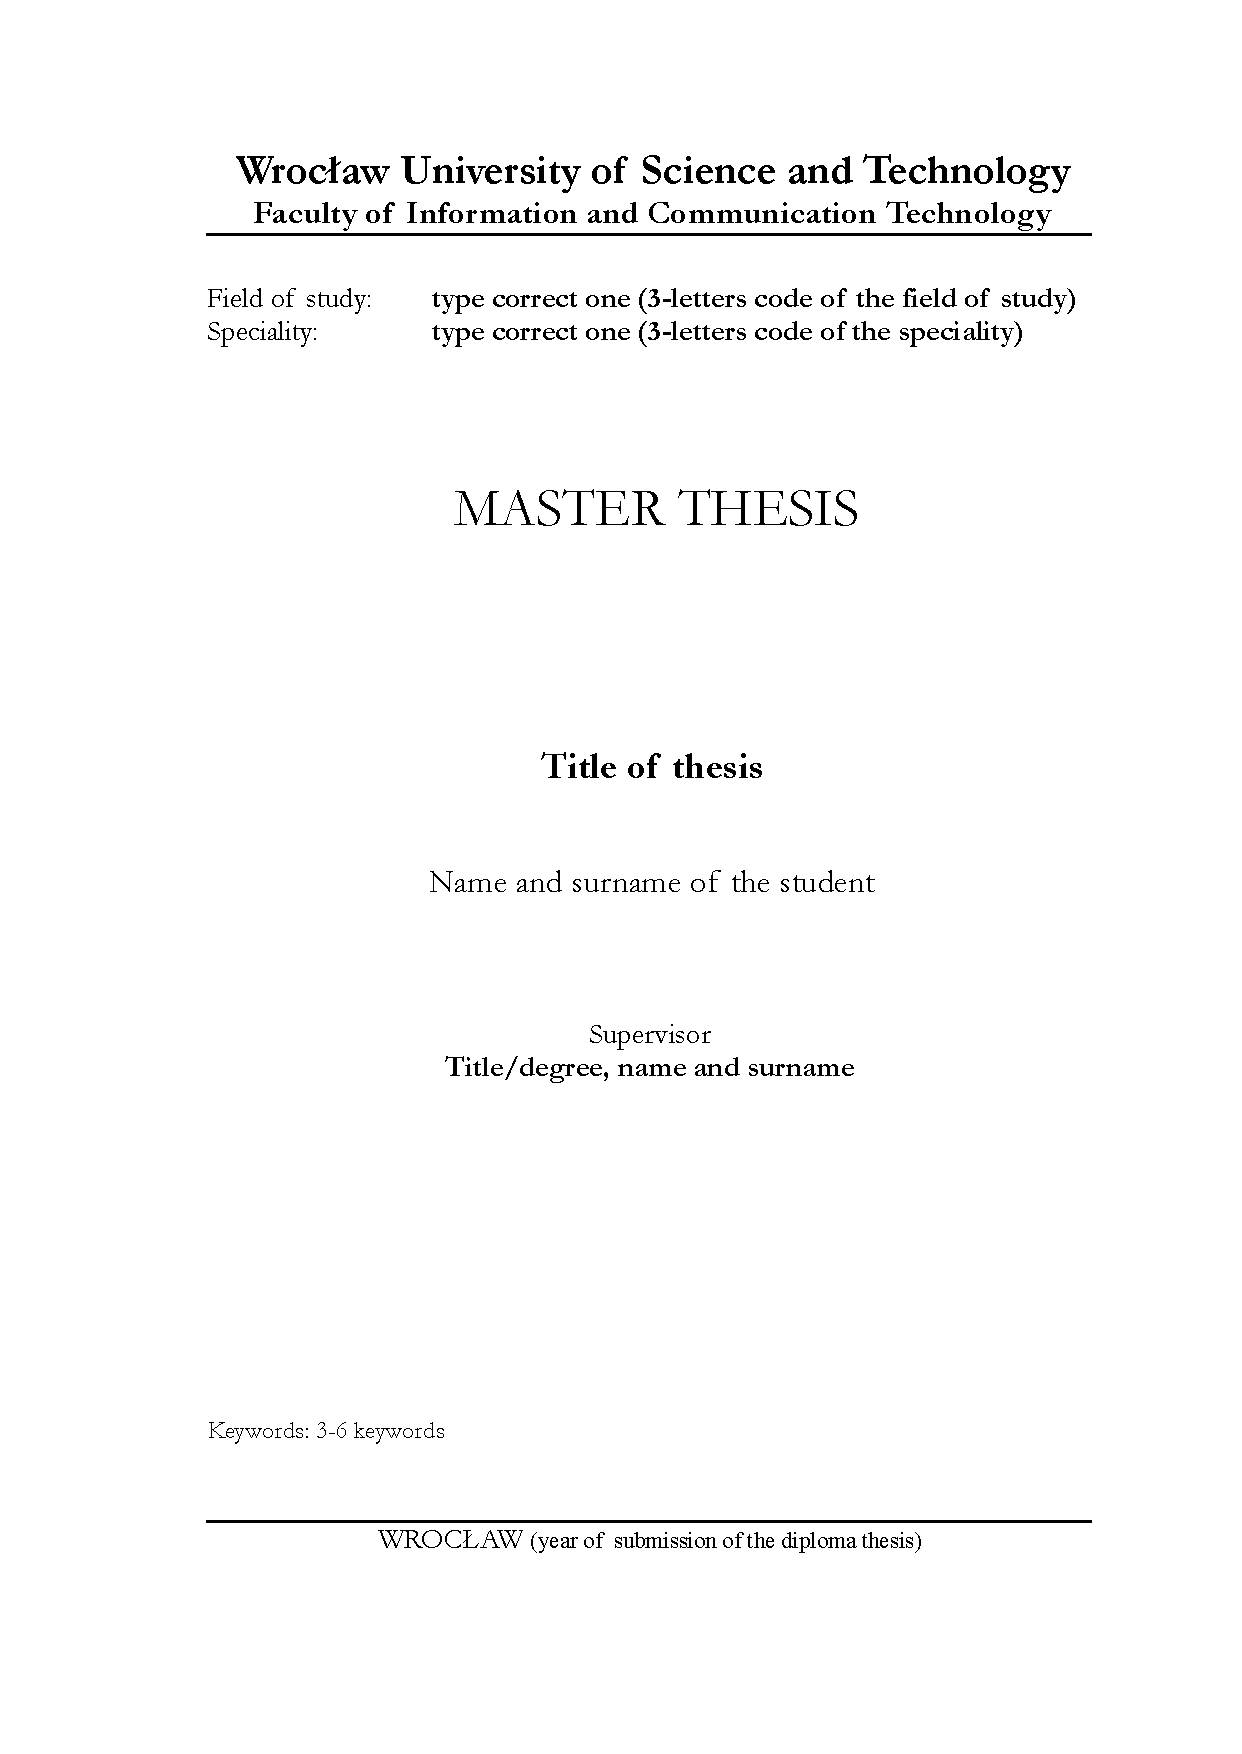
\includepdf[pages={1}]{title_page/pd_mgr_en.pdf}
\doublepage
% Add table of contents
\pagestyle{tableOfContentStyle}
% Add abstract
\pagenumbering{Roman}
\section*{Streszczenie}

Dodaj streszczenie pracy w języku polskim. Staraj się uwzględnić wymienione na stronie tytułowej słowa kluczowe. Uwaga przedstawiony rekomendowany szablon dotyczy pracy dyplomowej pisanej w języku angielskim. W przeciwnym wypadku, student powinien samodzielnie zmienić nazwy ,,Chapter'' na ,,Rodział'' itp stosując odpowiednie pakiety systemu \LaTeX oraz ustawienia w pliku \textit{latex-settings.tex}.

\section*{Abstract}

Streszczenie  w języku angielskim.
\doublepage
\tableofcontents
\doublepage
% Set page style 
\pagestyle{custom}
\mainmatter

% Create chapters:
\Chapter{Introduction}\label{chapter:introduction}
W pracy formułuje się cele o charakterze badawczym wymagające doboru i zastosowania metod badawczych, wykorzystując wiedzę teoretyczną oraz naukową. Wskazane jest przedstawienie, co nowego jest zaproponowane w pracy oraz podanie ograniczeń i słabych/mocnych stron opracowanego rozwiązania (jeżeli dotyczy). Rozdział wprowadzający powinien służyć czytelnikowi do zrozumienia celu pracy.

\section{Problem Statement}
W tej sekcji student powinien przedstawić bliżej problem, którym chce się zmierzyć. Jasno zdefiniuj problem badawczy. Podaj swoje cele, zadania i pytania badawcze. Wyjaśnij znaczenie badania. Określ ograniczenia badań.


\section{Thesis Objectives}
W tej sekcji powinny zostać przedstawione konkretne działania, które określają pracę studenta w celu rozwiązania problemu.


\section{Thesis Outline}
Zarysuj strukturę swojej pracy dyplomowej. Ogólnie przedstawienie pracy. Przykładowo: ,,Praca dzieli się na $7$ rozdziałów (\dots)''. Rozdział \ref{chapter:politechnika} dotyczy (\dots). Temat został rozwinięty~w~\ref{chapter:podrozdzial}.
\Chapter{Related Work}\label{chapter:related}
W tej sekcji powinny zostać przedstawione powiązane prace z tematem. Przedstaw tło i kontekst badań.

\section{Model Compression}

Dzięki technice X~\cite{nowak2016} uzyskujemy (\dots). Zgodnie ze standardem bibliografia powinna być uszeregowana alfabetycznie według haseł autorskich, dlatego może się zażyć, że wcześniejsze odwołanie ma wyższą cyfrę.

\section{XYZ}
XYZ używany jest do (\dots). Dzięki tej technice (\dots). Powstało wiele rozwinięć tematu takie jak (\dots)~\cite{nowak2018, w4n2017}, czy (\dots) \cite{babington2008}.

Zauważ, że strona pierwsza rozdziału ma inny styl niż kolejne. Rozdział powinien zawsze rozpoczynać się na nieparzystej stronie. Parzyste strony w nagłówku mają podkreślony wydział: ,,Faculty of Information and Communication Technology''; nieparzyste (z wyjątkiem pierwszych stron tytułowych): ,,Wrocław University of Science and Technology''. Jeśli rozdział kończy się na stronie nieparzystej powinna zostać dodana pusta strona bez formatowania, tak aby kolejny rozdział rozpoczynał się ponownie od strony nieparzystej. Jakkolwiek staramy się unikać pustych stron.
\Chapter{Politechnika Wrocławska}\label{chapter:politechnika}

Politechnika Wrocławska to państwowa uczelnia techniczna we Wrocławiu. Figure~\ref{fig:logo} przedstawia logo uczelni.

\begin{figure}[h]
    \centering
    
\includegraphics[width=0.9\textwidth]{images/LogoPWr.png}
    \caption{Logo Politechniki Wrocławskiej}\label{fig:logo}
\end{figure}

Pamiętaj by nie zostawiać pustych miejsc pod tytułem rozdziału. Należy pamiętać o wprowadzeniu. Dopiero później powinny zostać przedstawione podrozdziały.

\section{Tytuł podrozdziału}\label{chapter:podrozdzial}
Praca może zawierać także tabele, które powinny być czytelne i dobrze opisane. Do wszystkich tabel i rysunków powinny pojawić się odwołania w tekście (oraz komentarze). Podpisy rysunków mają znaleźć się pod rysunkami, a podpisy tabel – nad tabelami. Tabela~\ref{tab:tab_example} stanowi przykład.

\begin{table}[H]
    \centering
    \caption{Krótki ale treściwy opis tabeli} \label{tab:tab_example}
    \begin{tabular}{lrrrr}
        \toprule
        Method & anger          & joy            & optimism       & sadness        \\
        \midrule
        model1 & 0.772          & \textbf{0.751} & \textbf{0.532} & 0.673          \\
        model2 & 0.727          & 0.661          & 0.307          & 0.629          \\
        model3 & 0.761          & 0.739          & 0.498          & \textbf{0.679} \\
        model4 & \textbf{0.782} & 0.740          & 0.470          & 0.672          \\
        \bottomrule
    \end{tabular}
\end{table}

Warto także użyć gotowych generatorów do tabel (np. \url{https://www.tablesgenerator.com/}), niż formatować je samodzielnie. Mistrzem formatowania był Wojtek. Tabela~\ref{tab:main_results_sentence} o nieco zmienionej treści pochodzi z jego pracy.

\begin{table}[H]
    \centering
    \renewcommand*{\arraystretch}{1.3}
    \caption{Comparison of the compression methods considered for MultiEmo for the sentence level in the mixed domain scenario. The results are averaged on 5 repetitions. The best results are in \textbf{bold}.}
    \label{tab:main_results_sentence}
    \begin{tabular}{@{}
        l
        R{1.3cm}R{0.7cm}@{\hspace{0.1cm}}L{1.1cm}@{\hspace{8pt}}
        R{1.3cm}c@{\hspace{12pt}}
        cccc
        @{}}
        \toprule
        \multicolumn{1}{c}{\textbf{Method}}                                                                       &
        \multicolumn{1}{c}{\textbf{$\boldsymbol{\#}$Par.}}                                                        &
        \multicolumn{2}{c@{\hspace{12pt}}}{
        \begin{tabular}[c]{@{}c@{}}\textbf{Mem.}\\\textbf{ [MB]}\end{tabular}}  &
        \begin{tabular}[c]{@{}c@{}}\textbf{Train.}\\\textbf{ [min]}\end{tabular} &
        \textbf{Eval [s]}                                                                                         &
        \textbf{Acc.}                                                                                             &
        \textbf{F1}                                                                                               &
        \textbf{Rec.}                                                                                             &
        \textbf{Prec.}                                                                                                                                                                                                                                                                    \\
        \midrule
        Model$_\mathrm{BASE}$                                                                                     & 109M        & \multicolumn{2}{c@{\hspace{10pt}}}{418} & 26.0           & 13.9        & 78.8               & 74.7         & 74.1         & 75.8                        \\
        \midrule
        Model1                                                                                                    & 67M         & 255                                     & (1.6x)         & 14.1        & 7.0 (2.0x)         & 77.9         & 73.9         & 73.3         & \bftab{74.8} \\
        Model2                                                                                                    & \bftab{13M} & \bftab{49}                              & \bftab{(8.6x)} & 6.5         & 2.3 (6.2x)         & 76.7         & 72.4         & 71.7         & 73.9         \\
        Model3$_{6, \mathrm{TA}}$                                                                                 & 67M         & 255                                     & (1.6x)         & 14.1        & 7.2 (1.9x)         & 77.7         & 73.8         & 73.5         & 74.3         \\
        Model3$_{6, \mathrm{TS}}$                                                                                 & 68M         & 258                                     & (1.6x)         & 62.9        & 7.2 (1.9x)         & \bftab{78.2} & \bftab{74.4} & \bftab{74.1} & 74.7         \\
        Model3$_{4, \mathrm{TA}}$                                                                                 & 14M         & 55                                      & (7.6x)         & \bftab{5.5} & 2.1 (6.6x)         & 76.3         & 72.0         & 71.1         & 73.7         \\
        Model3$_{4, \mathrm{TS}}$                                                                                 & 15M         & 56                                      & (7.5x)         & 38.3        & \bftab{2.0 (6.9x)} & 76.3         & 72.2         & 71.5         & 73.4         \\
        Model4                                                                                                    & 67M         & 255                                     & (1.6x)         & 19.1        & 7.8 (1.8x)         & 76.6         & 72.5         & 72.1         & 73.2         \\
        Model5                                                                                                    & 14M         & 55                                      & (7.6x)         & 121.5       & 3.4 (4.1x)         & 77.5         & 72.9         & 72.2         & 74.9         \\
        \bottomrule
    \end{tabular}
\end{table}

\subsection{Tytuł podpodrozdziału}
Studia zapewniają podstawową wiedzę z zakresu sztucznej inteligencji i nauki o danych (data science). Rozwijają zarówno umiejętności matematyczne, programistyczne, obliczeniowe, analityczne, jak i umiejętności pracy projektowej w grupie, z nastawieniem na identyfikowanie problemów (naukowych, biznesowych, społecznych) i ich rozwiązywanie z wykorzystaniem technik i metod inteligentnych.

\section{Tytuł podrozdziału 2}
Społeczeństwo w swoim rozwoju wchodzi w czwartą rewolucję przemysłową, określaną często terminem ,,Przemysł 4.0''. Jest on oparty na systemach łączności piątej i wyższych generacji oraz Internecie Rzeczy (IoT), wspieranych sztuczną inteligencją.

Przemysł 4.0 zmienia nie tylko technologie, ale przede wszystkim model biznesu i wymagania stawiane pracownikom. Rewolucja oprze się na danych, które będą zbierane, gromadzone i przetwarzane na każdym etapie prowadzenia biznesu. W firmach wykorzystywane będą nowoczesne technologie, chmury obliczeniowe, wielkie zbiory danych, Internet Rzeczy, rozszerzona rzeczywistość, sztuczna inteligencja czy druk 3D.

Technologia powinna uwzględniać właściwe współdziałanie z człowiekiem. Dlatego należy badać aspekty komunikacji i interakcji człowiek – komputer czy szerzej: człowiek i rozbudowane środowiska robotyczne. Bariery rozwoju Przemysłu 4.0 mają związek przede wszystkim z dostępem do wykształconych kadr. To zrozumiałe w obliczu dużych oczekiwań co do interdyscyplinarnych kompetencji stawianych inżynierom.

Nauka przed wyzwaniami
Przyszłość stawia przed europejską nauką trzy kluczowe wyzwania:

\begin{itemize}
    \item Rozwój innowacji zakłócających – innowacje przełomowe, takie które zmienią istniejący porządek na rynku, wprowadzając coś zupełnie nowego.
    \item Biologizacja techniki – zastosowanie praw biologicznych, rządzących procesami zachodzącymi w organizmach żywych, do innych dziedzin.
    \item Bezpieczeństwo publiczne – nowe rozwiązania jakościowe i innowacje dotyczące: bezpieczeństwa w zakresie IT (m.in. w kontekście ataków cybernetycznych), bezpieczeństwa systemów transportu drogowego, kolejowego i lotniczego, bezpieczeństwa infrastrukturalnego miast i zaopatrzenia w wodę i elektryczność.
\end{itemize}

Badania i dydaktyka na wysokim poziomie
Szczególna rola w przełamywaniu barier rozwoju Przemysłu 4.0 przypadnie uniwersytetom, które w swoich zadaniach statutowych mają: badania naukowe i kształcenie na wysokim poziomie.
Zadania te są równie ważne. Nie ma bowiem wysokiej jakości nauczania bez prowadzenia badań naukowych. Nie ma badań naukowych i rozwoju gospodarki bez odpowiednio wykształconej kadry. To uczelnie będą przełamywały główne bariery czwartej rewolucji przemysłowej. Wśród tych uczelni – biorąc pod uwagę kapitał ludzki i społeczny, infrastrukturę badawczą i dydaktyczną – nie może zabraknąć Politechniki Wrocławskiej, aspirującej do bycia uczelnią badawczą. Te istotne zadania w pokonywaniu barier realizują wydziały. Na nie, a przede wszystkim na nowo powstały Wydział Informatyki i Telekomunikacji, spada odpowiedzialność w tej dziedzinie.

Wydział tworzą katedry pochodzące z wydziałów Politechniki Wrocławskiej: Elektroniki, Informatyki i Zarządzania oraz Podstawowych Problemów Techniki.
Badania naukowe prowadzone będą w katedrach: Automatyki, Mechatroniki i Systemów Sterowania, Informatyki Technicznej, Systemów i Sieci Komputerowych, Telekomunikacji i Teleinformatyki, Informatyki i Inżynierii Systemów, Informatyki Stosowanej, Inteligencji Obliczeniowej, Podstaw Informatyki.

Oznacza to, że swoim zakresem obejmą większość dziedzin bezpośrednio związanych z Przemysłem 4.0. Realizowane będą zarówno badania podstawowe, jak i wdrożeniowe, skupimy się także na aktywnej współpracy z gospodarką i komercjalizacji wyników. W/w katedry są gwarancją, że badania obejmą większość dziedzin bezpośrednio związanych z Przemysłem 4.0.

Za cel stawiamy sobie przede wszystkim zapewnienie przyjaznych warunków do rozwoju naukowego, zwłaszcza młodym, oraz przejrzystą ścieżkę kariery naukowej. Badania będziemy prowadzić we wszystkich dyscyplinach powiązanych z informatyką.

Kadra ma świadomość, że fundamentem wydziału jest – stojące na wysokim poziomie, nowoczesne, spełniające potrzeby zmieniającego się świata – nauczanie. Odbywać się ono będzie na 12 polsko- i anglojęzycznych kierunkach: Computer Science, Computer Security, Cyberbezpieczeństwo, Informatyczne Systemy Automatyki, Informatyka Algorytmiczna, Informatyka Stosowana, Informatyka Techniczna, Inżynieria Systemów, Sztuczna Inteligencja, Teleinformatyka, Telekomunikacja, Zaufane Systemy Sztucznej Inteligencji. Lista kierunków będzie sukcesywnie modyfikowana w odpowiedzi na wyzwania stawiane przez uwarunkowania społeczno-gospodarcze.

\Chapter{Conclusions and Future}\label{chapter:conclusions}
Zakończenie, podsumowuje najważniejsze wnioski, podaje możliwości dalszego rozwinięcia wykonanych prac i wskazuje obszar potencjalnego zastosowania pracy. Rezultaty pracy mają charakter poznawczy, mogą mieć charakter użytkowy. Należy dokonać analizy uzyskanych wyników. Rezultaty powinny charakteryzować się oryginalnością, a nawet w pewnym stopniu nowatorstwem. Praca zawiera (\dots). Zostało pokazane (\dots). Eksperymenty wykazały (\dots). Tu piszemy wnioski i obserwacje.

Widzimy, że (\dots). Z tego powodu przyszła praca powinna obejmować (\dots).
% Redefine plain for 1st bibliography page style
\resetformatting
% Please read :
%https://www.overleaf.com/learn/latex/Bibliography_management_with_bibtex
\pagestyle{bibliographyStyle}
\bibliographystyle{abbrv}
\bibliography{bibliography}

% Add list of figures and tables
\pagestyle{custom}
\newpage
\pagestyle{ListofFiguresStyle}
\listoffigures
\newpage
\pagestyle{ListofTablesStyle}
\listoftables
\end{document}